\documentclass[11pt]{article}

%\textheight 8.5in
%\topmargin -0.2in
%\oddsidemargin -0.20in
%\textwidth 6in
\textheight 8.5in
\topmargin -0.2in
\oddsidemargin -0.20in
\textwidth 6.3in
\flushbottom

\usepackage[colorlinks=true,linkcolor=blue,citecolor=blue]{hyperref}
\usepackage{bm}
\usepackage{algorithm}
\usepackage{algpseudocode}
\usepackage{amsmath}
\usepackage{bbm}
\usepackage{cite}
\usepackage{makecell}
\usepackage{amsfonts}
\usepackage{amssymb}
\usepackage{amsthm}
\usepackage{fancybox}
\usepackage{multirow}
\usepackage{tikz}
\usepackage{thm-restate}
\usepackage{wrapfig}
\usepackage{mathtools}
\usepackage{booktabs}
\usepackage{tikz}
%% Theorems
\newtheorem{theorem}{Theorem}[section]
\newtheorem{corollary}[theorem]{Corollary}
\newtheorem{lemma}[theorem]{Lemma}
\newtheorem{definition}{Definition}
\newtheorem{problem}{Problem}
\newtheorem{fact}{Fact}
\newtheorem*{lemma*}{Lemma}

%% Linear Algebra
\newcommand{\tran}[0]{\ensuremath{^{\mathsf{T}}}\xspace}
\newcommand{\mat}[1]{\boldsymbol{#1}}
\renewcommand{\vec}[1]{\boldsymbol{#1}}
\providecommand{\eye}{\ensuremath{\mat{I}}}
\providecommand{\mA}{\ensuremath{\mat{A}}}
\providecommand{\mB}{\ensuremath{\mat{B}}}
\providecommand{\mC}{\ensuremath{\mat{C}}}
\providecommand{\mD}{\ensuremath{\mat{D}}}
\providecommand{\mE}{\ensuremath{\mat{E}}}
\providecommand{\mF}{\ensuremath{\mat{F}}}
\providecommand{\mG}{\ensuremath{\mat{G}}}
\providecommand{\mH}{\ensuremath{\mat{H}}}
\providecommand{\mI}{\ensuremath{\mat{I}}}
\providecommand{\mJ}{\ensuremath{\mat{J}}}
\providecommand{\mK}{\ensuremath{\mat{K}}}
\providecommand{\mL}{\ensuremath{\mat{L}}}
\providecommand{\mM}{\ensuremath{\mat{M}}}
\providecommand{\mN}{\ensuremath{\mat{N}}}
\providecommand{\mO}{\ensuremath{\mat{O}}}
\providecommand{\mP}{\ensuremath{\mat{P}}}
\providecommand{\mQ}{\ensuremath{\mat{Q}}}
\providecommand{\mR}{\ensuremath{\mat{R}}}
\providecommand{\mS}{\ensuremath{\mat{S}}}
\providecommand{\mT}{\ensuremath{\mat{T}}}
\providecommand{\mU}{\ensuremath{\mat{U}}}
\providecommand{\mV}{\ensuremath{\mat{V}}}
\providecommand{\mW}{\ensuremath{\mat{W}}}
\providecommand{\mX}{\ensuremath{\mat{X}}}
\providecommand{\mY}{\ensuremath{\mat{Y}}}
\providecommand{\mZ}{\ensuremath{\mat{Z}}}
\providecommand{\mLambda}{\ensuremath{\mat{\Lambda}}}
\providecommand{\mSigma}{\ensuremath{\mat{\Sigma}}}
\providecommand{\vone}{\ensuremath{\vec{1}}}
\providecommand{\vzero}{\ensuremath{\vec{0}}}
\providecommand{\va}{\ensuremath{\vec{a}}}
\providecommand{\vb}{\ensuremath{\vec{b}}}
\providecommand{\vc}{\ensuremath{\vec{c}}}
\providecommand{\vd}{\ensuremath{\vec{d}}}
\providecommand{\ve}{\ensuremath{\vec{e}}}
\providecommand{\vf}{\ensuremath{\vec{f}}}
\providecommand{\vg}{\ensuremath{\vec{g}}}
\providecommand{\vh}{\ensuremath{\vec{h}}}
\providecommand{\vi}{\ensuremath{\vec{i}}}
\providecommand{\vj}{\ensuremath{\vec{j}}}
\providecommand{\vk}{\ensuremath{\vec{k}}}
\providecommand{\vl}{\ensuremath{\vec{l}}}
\providecommand{\vm}{\ensuremath{\vec{l}}}
\providecommand{\vn}{\ensuremath{\vec{n}}}
\providecommand{\vo}{\ensuremath{\vec{o}}}
\providecommand{\vp}{\ensuremath{\vec{p}}}
\providecommand{\vq}{\ensuremath{\vec{q}}}
\providecommand{\vr}{\ensuremath{\vec{r}}}
\providecommand{\vs}{\ensuremath{\vec{s}}}
\providecommand{\vt}{\ensuremath{\vec{t}}}
\providecommand{\vu}{\ensuremath{\vec{u}}}
\providecommand{\vv}{\ensuremath{\vec{v}}}
\providecommand{\vw}{\ensuremath{\vec{w}}}
\providecommand{\vx}{\ensuremath{\vec{x}}}
\providecommand{\vy}{\ensuremath{\vec{y}}}
\providecommand{\vz}{\ensuremath{\vec{z}}}
\providecommand{\vchi}{\ensuremath{\vec{\chi}}}
\providecommand{\vpsi}{\ensuremath{\vec{\psi}}}
\providecommand{\vpi}{\ensuremath{\vec{\pi}}}
\providecommand{\vlambda}{\ensuremath{\vec{\lambda}}}
\providecommand{\vdelta}{\ensuremath{\vec{\delta}}}
\providecommand{\vepsilon}{\ensuremath{\vec{\epsilon}}}
\newcommand{\norm}[1]{\left\lVert #1\right\rVert}
\newcommand{\bmat}[1]{\begin{bmatrix} #1 \end{bmatrix}}

\newcommand{\Z}{\ensuremath{\mathbb{Z}}}
\newcommand{\vol}{\mathrm{Vol}}
\newcommand{\R}{\mathbb{R}}
\newcommand{\Sbar}{\bar{S}}

\title{A Cheeger Inequality for Size-Specific Conductance}

% \author{
% % Anonymous Authors
% % }
\author{
Yufan Huang\\
Purdue University\\
\texttt{huan1754@purdue.edu}
% \and C. Seshadhri\\
% University of California, Santa Cruz\\
% \texttt{sesh@ucsc.edu}
\and
David F.~Gleich\\
Purdue University \\
\texttt{dgleich@purdue.edu}
}

\newcommand\blfootnote[1]{%
  \begingroup
  \renewcommand\thefootnote{}\footnote{#1}%
  \addtocounter{footnote}{-1}%
  \endgroup
}

\begin{document}
\maketitle

\begin{abstract}
    The \(\mu\)-conductance measure proposed by Lovasz and Simonovits is a size-specific conductance
    score that identifies the set with smallest conductance while disregarding those sets with
    volume smaller than a \(\mu\) fraction of the whole graph. Using \(\mu\)-conductance enables us
    to study in new ways. In this manuscript we propose a modified spectral cut that is a natural
    relaxation of the integer program of \(\mu\)-conductance and show the optimum of this program
    has a two-sided Cheeger inequality with \(\mu\)-conductance.  \blfootnote{This is a working
      paper that documents the details of a simple technical result. In may be incorporated into a
      future paper for the purposes of publication. The work was funded in part by NSF CCF-1909528,
      IIS-2007481, DOE DE-SC0023162, and the IARPA Agile program. We thank C.~Seshadhri for
      discussions on this topic.}
\end{abstract}


%\newpage
\section{Conductance and the Cheeger Inequality}
    %The Cheeger inequality gives a two-sided bound to the set of best conductance in a graph via an
    %eigenvector computation~\cite{Chung-2007-four,cheeger69}.

    
    
    Consider an undirected graph \(G = (V, E, w : E \to \R)\) with \(n\) vertices and \(m\) edges,
    the degree of a vertex \(v\) is the sum of weights of edges adjacent to it, in other words
    \(d(v) = \sum_{u \in V} w(v, u)\) where \(w(v, u)\) is the weight of edge \(vu\) and for an
    non-existing edge, we have its weight being zero.
    
    For a set \(S \subset V\), we let 
    \[\vol(S) = \sum_{v \in S} d(v)\]
    denote the volume of set \(S\) which is a well-known size measure of a vertex set, and we let
    \[\partial S = \{uv \in E: u \in S, v \in \Sbar \}\]
    denote the cut between \(S\) and \(\Sbar \coloneqq V \setminus S \) and 
    \[|\partial S| = \sum_{uv \in \partial S} w(u, v) \] 
    denote the size of cut \(\partial S\). 
    The conductance of \(S\),  
    \[ \phi(S) = \frac{|\partial S| }{\min\{\vol(S), \vol(\Sbar)\}}\]
    measures how well-connected the set $S$ is to the rest of the graph. Further, the conductance of $G$,
    \[
        \phi(G) = \min_{S \subset V} \phi(S) 
    \]
    takes the minimum over all possible $S$ and characterizes how well-connected the whole graph is.

    For a graph, its degree matrix $\mD$ is the diagonal matrix with $\mD_{vv} = d(v)$ and its graph
    Laplacian matrix $\mL$ is defined as
    \[\mL = \sum_{vu \in E} w(v, u) (\vone_{u} - \vone_{v}) (\vone_{u} - \vone_{v})^T.\] 
    where \(\vone_S\) is the indicator vector for set \(S\) and we write \(\vone_{a}\) in short for
    \(\vone_{\{a\}}\).

    The Cheeger inequality gives a two-sided bound to the set of best conductance in a graph via an
    eigenvector computation of its graph Laplacian~\cite{cheeger69, Chung-2007-four}. It says
    \[
        2\phi(G) \geq  \lambda_2 \geq \frac12 \phi(G)^2 
    \]
    where \(\lambda_2\) is the second smallest eigenvalue of the normalized Laplacian \( \mD^{-1/2}
    \mL \mD^{-1/2}\). This classical result bridges the gap between spectral theory and
    combinatorics and enable us to study the combinatoric structures of a graph via algebraic tools.
\section{Cheeger Inequality for $\mu$-conductance}
As a metric conductance captures only a single structure in a graph---the set with the worst
bottleneck. The size-specific $\mu$-conductance value has the potential to be sensitive to multiple
sets. We first provide one modified spectral program inspired by \(\mu\)-conductance and then
theoretically show that its optimum has a two-sided Cheeger inequality with \(\mu\)-conductance.

\subsection{The definition of \(\mu\)-conductance}

The idea of \(\mu\)-conductance is a parameterized variant of conductance that arises from Markov
chain theory \cite{Lovasz-1990-mixing}. Basically it computes the best set with smallest conductance
disregarding those sets with volume smaller than \(\mu \vol(G)\). Formally, it is defined as \footnote{Here we adopt a slightly different definition from the original paper. They are similar in spirit as they both neglect sets with volume smaller than a specific volume but the original one involves a perturbed conductance.} 
\begin{equation}
\phi_\mu(G) = \!\begin{array}[t]{l@{\,\,\,}l} \displaystyle \mathop{\text{minimize}}_{S \subset V} &
\phi(S) \\ \text{subject to} & \mu \vol(G) \! \le \! \vol(S) \! \le \! (1-\mu)\vol(G).  \end{array}
\label{eq:mu-cond}
\end{equation}
In the notation of \(\mu\)-conductance, the original conductance $\phi(G)$ can be expressed as
\(\phi_0(G)\).  So by computing \(\mu\)-conductance for multiple \(\mu\)s, we may be able gain
additional information about a graph.  This will only be productive is $\phi(G)$ arises \emph{only}
from a small set in the graph. If $\phi(G)$ arises from a set of nearly $\vol(G)/2$, then there are
no differences between conductance and $\mu$-conductance.

\subsection{A spectral program for $\mu$-conductance}

Before we introduce our modified spectral program for \(\mu\)-conductance, let us first revisit the
relation between conductance and spectral cut to smooth the transition to our new
program. Basically, the problem of finding the set of smallest conductance is equivalent to (up to a
constant factor) the following integer program
\begin{equation}
\begin{split}
\label{eq:conductance-ip}
  \displaystyle \mathop{\text{minimize}}_{S \subset V} & \quad \frac{\vpsi^T \mL \vpsi}{\vpsi^T \mD
    \vpsi} \\ \text{subject to} & \quad \vpsi = \frac{1}{\vol(S)} \vone_S - \frac{1}{\vol(\Sbar)}
  \vone_{\Sbar}.
\end{split}
\end{equation}
So the spectral cut 
\begin{align}
\begin{split}
\label{eq:conductance-spectral}
  \displaystyle \mathop{\text{minimize}}_{\vx \in \R^{|V|} } & \quad \frac{\vx^T \mL \vx}{\vx^T \mD
    \vx} \\ \text{subject to} & \quad \vx^T \vd = 0.
\end{split}
\end{align}
is actually a relaxation of \eqref{eq:conductance-ip} by replacing \(\vpsi\) with vectors orthogonal
to $\vd$.

This inspires us to begin with considering the following integer program of \(\mu\)-conductance
\begin{equation}
\begin{split}
\label{eq:mu-conductance-ip}
\displaystyle \mathop{\text{minimize}}_{S \subset V} \quad & \vpsi^T \mL \vpsi \\
\text{subject to} \quad & \vpsi = \sqrt{\frac{\vol(\Sbar)}{\vol(S)\vol(G)}} \vone_S -
\sqrt{\frac{\vol(S)}{\vol(\Sbar) \vol(G)}} \vone_{\Sbar} \\
& \vpsi^T \mD \vpsi = 1 \\
& \mu \vol(G) \le \vol(S) \le (1 - \mu) \vol(G).
\end{split}
\end{equation}
The difference between \eqref{eq:mu-conductance-ip} and \eqref{eq:conductance-ip} is that we add one
constraint on volume of \(S\) and we notice that \eqref{eq:conductance-ip} is scale-invariant with
regard to \(\vpsi\), therefore we re-scale \(\vpsi\) to make it satisfy \(\vpsi \mD \vpsi = 1\).
Notice that the constraint \(\mu \vol(G) \! \le \! \vol(S) \! \le \! (1 - \mu) \vol(G) \) implies
that the entries of \(\vpsi\) must be delocalized, in other words there will be no entries with very
large magnitude and no entries with very small magnitude. This integer problem can be relaxed to the
following spectral program
\begin{align}
\label{eq:mu-conductance-spectral}
\begin{split}
  \lambda_\mu = \displaystyle \mathop{\text{minimize}}_{\vx \in \R^{|V|} } \quad & \vx^T \mL \vx \\
\text{subject to} \quad &  \vx^T \vd = 0 \\
                        &  \vx^T \mD \vx = 1 \\
                        &  \|\vx\|_{\infty} \leq \sqrt{\frac{1 - \mu}{\mu \vol(G)}} \\ 
                        &  |\vx|_i \geq \sqrt{\frac{\mu}{(1 - \mu) \vol(G)}}, \quad \forall i \in V.  
\end{split}
\end{align}

\subsection{Main Result}
In this section, we demonstrate that a non-trivial relation is preserved by the relaxation from
\eqref{eq:mu-conductance-ip} to \eqref{eq:mu-conductance-spectral} and the optimum of spectral
program \eqref{eq:mu-conductance-spectral} has one two-sided Cheeger inequality with
\(\mu\)-conductance. Our main result is the following Theorem.
\begin{theorem}
\label{thm:cheeger}
Given a graph \(G\) and a constant \(0 \leq \mu \leq 1/2\), we have 
\[
2 \phi_\mu \ge \lambda_\mu \ge \frac12 
\max \left\{
   \min \left\{ \left( \frac{\mu}{1 - \mu} \phi_\mu \right)^2,
      \left(\frac{\mu^2 \phi_\mu + (1 - 2\mu) \phi_0}{1 - \mu - \mu^2} \right)^2 \right\}
      , \left(\phi_0 \right)^2 \right \}.
\]
\end{theorem}
Here for simplicity we make the assumption that there always exists one set \(S\) with volume
between \(\mu \vol(G)\) and \((1 - \mu) \vol(G)\), otherwise discussing \(\mu\)-conductance for this
specific \(\mu\) is meaningless.

Now before we start proving our main theorem, let us first introduce a few algebraic identities
which will simplify our proof.

\begin{lemma}
\label{lem:average-geq-least}
For non-negative \(a_i, b_i\), we have 
\[
\max_i \frac{a_i}{b_i} \ge \frac{\sum_{i} a_i}{\sum_{i} b_i} \ge \min_i \frac{a_i}{b_i}.
\]
\end{lemma}

\begin{lemma}
\label{lem:minmax-frac}
For a non-negative sequence \( \{x_i\}_{i=1}^k \) with bounded elements, in
otherwords  \(a \ge x_i \ge b \ge 0,  \forall i \in [k] \)   , and non-negative \(A, B,
\{c_i\}_{i=1}^k\), we have
\[\frac{A}{B + b \sum_{i=1}^k c_i} \ge \frac{A}{B + \sum_{i=1}^k c_ix_i } \ge \frac{A}{B + a \sum_{i=1}^k c_i}.\]
Further, for non-negative \(\{d_i\}_{i=1}^k\), if \(A - a \sum_{i=1}^k d_i \ge 0\), we have
\[\frac{A - b \sum_{i=1}^k d_i }{B + b \sum_{i=1}^k c_i } \ge \frac{A - \sum_{i=1}^k d_i x_i}{B + \sum_{i=1}^k c_i x_i} \ge \frac{A - a \sum_{i=1}^{k} d_i}{B + a \sum_{i=1}^k c_i}.\]
\end{lemma}

\begin{lemma}
    \label{lem:two-var-frac}
    For two non-negative variables \(X, Y\) with bounded ratio, in other words, \(b \ge \frac{X}{Y}
    \ge a \ge 0\), and non-negative constants \(A, B, C, D\), we have
    \[ \frac{AX + BY}{CX + DY} \ge \min \left\{ \frac{Ab + B}{Cb + D}, \frac{Aa + B}{Ca + D} \right\}.\]
\end{lemma}
The three Lemmas above can be verified with straightforward algebra. 
Also, we have the following fact.
\begin{fact}
\label{fac:lambda-mu-geq-phi0-sqr}
    \(\lambda_\mu \ge \phi_0^2/2. \)
\end{fact}
This is due to the observation that when \(\mu = 0\), \eqref{eq:mu-conductance-spectral} degenerates
to \eqref{eq:conductance-spectral} and \(\lambda_\mu\) is non-decreasing with regard to \(\mu\).

We split the proof of Theorem~\ref{thm:cheeger} into two parts, lower bound of \(\lambda_\mu\) and
upper bound of \(\lambda_\mu\).

\subsection{Proof for upper bound of \(\lambda_\mu\)}
We prove the following Lemma, see also~\cite{HSG23}. 
\begin{lemma}
\label{lem:cheeger-upper-bound}
    Given a graph \(G\) and a constant \(0 \le \mu \le 1/2\), we have
    \[2 \phi_\mu \ge \lambda_\mu.\]
\end{lemma}
\begin{proof}
    Let \(S\) be the vertex set which achieves the optimal \(\mu\)-conductance. By our relaxation, we know 
    \[
    \vpsi = \sqrt{\frac{\vol(\Sbar)}{\vol(S)\vol(G)}} \vone_S - \sqrt{\frac{\vol(S)}{\vol(\Sbar)
        \vol(G)}} \vone_{\Sbar}
    \]
    is naturally in the feasible region of \eqref{eq:mu-conductance-spectral}. Then, we have the
    corresponding objective value is
    \begin{align*}
         \vpsi^T \mL \vpsi 
    &= \frac{| \partial S| \vol(G)}{\vol(S) \vol(\Sbar)} \\
    &\leq  \frac{2 |\partial S|}{\min \{\vol(S), \vol(\Sbar) \}} \\
    &= 2 \phi_{\mu},
    \end{align*}
    which implies \(\lambda_\mu \le 2 \phi_\mu\). 
\end{proof}
We can see the proof above is a direct result of the relaxation. 

\subsection{Proof for lower bound of \(\lambda_\mu\)}

Now we arrive at the challenging part of the proof, lowering bounding \(\lambda_\mu\) via
\(\phi_\mu\). Our proof is mainly inspired by the proof in \cite{Chung-2007-four}. The first part of
our proof is exactly same, we restate it here for completeness.

Let \(\vg\) denote the vector that achieves the optimum of \eqref{eq:mu-conductance-spectral}. We
order all vertices such that \(\vg(v_1) \ge \vg(v_2) \ge \cdots \ge \vg(v_n)\) and denote \(S_j =
\{v_i \mid i \in [j]\}\) for \(\forall j \in [n]\), in other words \(S_j\) is the set of first \(j\)
vertices.

Then, we decompose $\vg$ into its positive components and negative components, denoted by $\vg_+$
and $\vg_-$ where
\begin{align*}
    \vg_+(v_i) &= \max(\vg(v_i), 0), \\
    \vg_-(v_i) &= \max(-\vg(v_i), 0).
\end{align*}
 We have 
 \begin{align*}
   \vg & = \vg_+ - \vg_-, \\  
   \vg(v_i)^2 &= \vg_+(v_i)^2 + \vg_-(v_i)^2, \forall i \in [n].
 \end{align*}
This is slightly different from the decomposition of $\vg$ in \cite{Chung-2007-four}. 

Define 
\[R(\vx) = \frac{\vx^T \mL \vx}{\vx^T \mD \vx}, \quad \forall \vx \in \R^V .\] We have 
\begin{equation}
\begin{split}
    R(\vg) &= \frac{\sum_{uv \in E}(\vg(u) - \vg(v))^2}{\sum_{v \in V} d(v) \vg(v)^2} \\ &\ge
    \frac{\sum_{uv \in E}(\vg_+(u) - \vg_+(v))^2 + \sum_{uv \in E}(\vg_-(u) - \vg_-(v))^2}{\sum_{v
        \in V} d(v) \vg(v)^2} \\ &= \frac{\sum_{uv \in E}(\vg_+(u) - \vg_+(v))^2 + \sum_{uv \in
        E}(\vg_-(u) - \vg_-(v))^2}{\sum_{v \in V} d(v) \vg_+(v)^2 + \sum_{v \in V} d(v)
      \vg_-(v)^2}\\ & \ge \min\{R(\vg_+), R(\vg_-)\}
           \label{eq:rayleigh-line4}.
\end{split}
\end{equation}
where in the first inequality we use the fact that \((\vg(u) - \vg(v))^2 \ge (\vg_+(u) - \vg_+(v))^2
+ (\vg_-(u) - \vg_-(v))^2\) and the in the second inequality we use
Lemma~\ref{lem:average-geq-least}.

Without loss of generality, we assume \(R(\vg_+)\) is smaller. Notice that 
\begin{align}
        R(\vg_+) &= \frac{\sum_{uv \in E} (\vg_+(u) - \vg_+(v))^2 \sum_{uv \in E} (\vg_+(u) +
          \vg_+(v))^2}{\sum_{v \in V} d(v) \vg_+(v)^2 \sum_{uv \in E} (\vg_+(u) + \vg_+(v))^2 }
        \nonumber \\ &\ge \frac{\left(\sum_{uv \in E} (\vg_+(u)^2 - \vg_+(v)^2) \right)^2
        }{2\left(\sum_{v \in V} d(v) \vg_+(v)^2 \right)^2 }\nonumber \\ & = \frac{\left(\sum_{i =
            1}^{n-1} (\vg_+(v_i)^2 - \vg_+(v_{i+1})^2) |\partial S_i| \right)^2} {2
          \left(\sum_{i=1}^{n} \vg_+(v_i)^2 d(v_i)\right)^2}.  \tag{a} \label{eq:case1-mid1}
\end{align}
where in the first inequality we use Cauchy-Schwarz inequality and AM-GM inequality, the second
equality is by re-arranging summations.

To this point, our proof is exactly the same with \cite{Chung-2007-four} except how we decompose
\(\vg\). But here we notice that we can not simply lower bound \(|\partial S_i|\) via \(\phi_0 \cdot
\min\{ \vol(S_i), \vol(\bar{S_i}) \}\) because then the lower bound is not related to
\(\phi_\mu\). Instead, we need to lower bound \(|\partial S_i| \) of those \(S_i\)s with \(\min\{
\vol(S_i), \vol(\bar{S_i}) \} \ge \mu \vol(G) \) by \(\phi_\mu \cdot \min\{ \vol(S_i),
\vol(\bar{S_i}) \}\), and \(|\partial S_i| \) of other \(S_i\)s by \(\phi_0 \cdot \min\{ \vol(S_i),
\vol(\bar{S_i}) \}\). This involves some case-by-case analysis.

Let us first introduce three important indices that appear repeatedly in our following proof. They
are summarized in Table~\ref{tab:indices}. We begin with one Lemma revealing the relation between
these three indices.
\begin{table}
    \centering
    \caption{Three key indices in our proof.}
    \begin{tabular}{rcl}
    \toprule 
   Index & Definition& Interpretation \\ 
    \midrule 
   $h$  & largest integer such that $\vol(S_h) \le \vol(G)/2$ & \emph{half} fraction of volume\\
   $u$  & largest integer such that $\vol(S_u) < \mu \vol(G)$ & 
   \emph{$\mu$} fraction of volume\\ 
   $z$  & largest integer such that $\vg(z) > 0$ & 
   $z + 1$ is \emph{zero point} of $\vg_+$\\ 
    \bottomrule
    \end{tabular}
    
    \label{tab:indices}
\end{table}

\begin{lemma}
\label{lem:relation-h-u-z}
By definition of $h, u, z$, we have 
\begin{enumerate}
    \item $u \le h$,
    \item $\vol(S_z) \in [\mu \vol(G), (1 - \mu) \vol(G)]$,
    \item $u < z$. 
\end{enumerate}
\end{lemma}
\begin{proof}
\begin{enumerate}
    \item Since $\mu \le 1/2$, we have $u \le h$ by definition. 
    \item We prove $\vol(S_z) \ge \mu \vol(G)$ by contradiction.   
Assume $\vol(S_z) < \mu\vol(G)$. Notice
\[
  \sum_{i=1}^n \vg(v_i) d(v_i) = \sum_{i=1}^{z} \vg(v_i) d(v_i) + 
  \sum_{i=z+1}^n \vg(v_i) d(v_i)
\]
where $\vg(v_i) > 0$ for $\forall i \in [z]$ and $\vg(v_i) \le 0$ for other $i$s. Therefore because
of the last two constraints of \eqref{eq:mu-conductance-spectral}, we have
\begin{align*}
  \sum_{i=1}^n \vg(v_i) d(v_i) &\leq \sum_{i=1}^{z} \sqrt{\frac{1 - \mu}{\mu \vol(G)}} d(v_i)
  - \sum_{i=z+1}^n \sqrt{\frac{\mu}{(1-\mu) \vol(G)}} d(v_i)  \\
   &= \sqrt{\frac{1 - \mu}{\mu \vol(G)}} \vol(S_z)
  - \sqrt{\frac{\mu}{(1-\mu) \vol(G)}} \vol(\bar{S}_z)\\
   & <  \sqrt{\frac{1 - \mu}{\mu \vol(G)}} \mu \vol(G) - \sqrt{\frac{\mu}{(1-\mu) \vol(G)}} (1 - \mu) \vol(G) 
   \\
   & = 0  
\end{align*}
which contradicts $\vg$ is a \emph{valid} solution of \eqref{eq:mu-conductance-spectral}. 

By symmetry, we can prove that $\vol(S_z) \le (1 - \mu) \vol(G)$ similarly.
\item This follows directly from the fact that $\vol(S_u) < \mu \vol(G) \le \vol(S_z)$. 
\end{enumerate}
\end{proof}

\begin{figure}
\centering
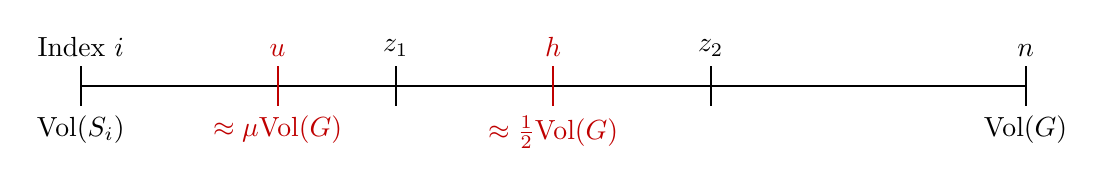
\begin{tikzpicture}[scale=1]
    \draw[line width = 0.25mm] (0,0) -- (12,0) ; 
    \draw[line width = 0.25mm,red!75!black] (6, -0.25) -- (6, 0.25) node [above] {$h$} node [below = 0.5cm ] {$\approx \frac12 \vol(G)$}; 
    \draw[line width = 0.25mm] (0, -0.25) -- (0, 0.25) node [above] {Index $i$} node [below = 0.5cm] {$\vol(S_i)$}; 
    \draw[line width = 0.25mm] (12, -0.25) -- (12, 0.25) node [above] {$n$} node [below = 0.5cm ] {$\vol(G)$}; 
    \draw[line width = 0.25mm,red!75!black] (2.5, -0.25) -- (2.5, 0.25) node [above] {$u$} node [below = 0.5cm ] {$\approx \mu\vol(G)$}; 
    \draw[line width = 0.25mm] (4, -0.25) -- (4, 0.25) node [above] {$z_1$}; 
    \draw[line width = 0.25mm] (8, -0.25) -- (8, 0.25) node [above] {$z_2$}; 
\end{tikzpicture}
\caption{Relative positioning of indices \(u, h, z\) and the volumes of \(S_u, S_h\). There are two
  possible positions for $z$. Here \(z_1\) corresponds to the case \(z < h\) discussed in
  Lemma~\ref{lem:case1} and \(z_2\) corresponds to the case \(h \le z\) discussed in
  Lemma~\ref{lem:case2}.}
\label{fig:index-rel-pos}
\end{figure}

Figure~\ref{fig:index-rel-pos} summarizes what we show in Lemma~\ref{lem:relation-h-u-z}. Now we
divide the discussion into two cases based on the magnitude of $h$ and $z$. The difference is that
if $h \ge z$, then for any $i$ such that $\vg_+(v_i) > 0$, we have $\vol(S_i) \le \vol(G) / 2$,
which implies $\min \{\vol(S_i), \vol(\bar{S}_i)\} = \vol(S_i)$ always holds. But if $h < z$, then
for those $i \in (h, z]$, we have $\vg_+(v_i) > 0$ and $\min \{\vol(S_i), \vol(\bar{S}_i)\} =
  \vol(\bar{S}_i) = \vol(G) - \vol(S_i)$, which makes the analysis more complex.

For convenience, we let 
\begin{align*}
   \vp_i &= \vg_+(v_i)^2, \forall i \in [n] \\ 
   \vdelta_i &= \vp_i - \vp_{i+1}, \forall i \in [n-1]. 
\end{align*}
By definition, both \(\vp\) and \(\vdelta\) are non-negative and elements of \(\vp\) are non-increasing. 

For the case \(h \geq z\), we have the following Lemma. 
\begin{lemma}
\label{lem:case1}
    If \(h \geq z\), then we have
    \[R(\vg_+)  \ge \frac{1}{2} \left(\frac{\mu^2}{(1-\mu)^2} \phi_\mu + \frac{1 - 2\mu}{(1 - \mu)^2} \phi_0 \right)^2.\]
\end{lemma}
\begin{proof}
   In this case for any $i \leq z, \vol(S_i) \leq \vol(\bar{S_i})$. Using the relationship among $h,
   u, z$, which is $u < z \le h$, we get
   \begin{align}
        R(\vg_+) \ge \eqref{eq:case1-mid1} &= \frac12 \left(\frac{\sum_{i = 1}^{z} \vdelta_i |\partial S_i| } 
             { \sum_{i=1}^{z} \vp_i d(v_i)} \right)^2 \nonumber \\
            &= \frac12 \left(\frac{\sum_{i=1}^u \vdelta_i |\partial S_i| 
               + \sum_{i=u+1}^z \vdelta_i |\partial S_i| }
               {\sum_{i=1}^{z} \vp_i d(v_i)} \right)^2 \nonumber \\
            &\geq \frac12 \left(\frac{\phi_0 \sum_{i=1}^u \vdelta_i  \vol(S_i) 
               + \phi_\mu\sum_{i=u+1}^z \vdelta_i \vol(S_i) }
               {\sum_{i=1}^{z} \vp_i d(v_i)} \right)^2 \tag{b} \label{eq:case1-mid2}
   \end{align}
   where in the last inequality we use the definitions of index \(u\) and conductance.
   By writing out the summation and offsetting by one, we notice 
   \begin{align}
   \sum_{i=1}^u \vdelta_i \vol(S_i) &= \left( \sum_{i=1}^{u} \vp_i d(v_i) \right) - \vp_{u+1} \vol(S_u) \nonumber  \\
    &= \sum_{i=1}^u \left(\vp_i - \vp_{u+1}\right) d(v_i) \nonumber 
   \end{align}
   and
   \begin{align*}
    \sum_{i=u+1}^z \vdelta_i \vol(S_i) &= 
 \vp_{u+1} \vol(S_{u+1}) + \sum_{i=u+2}^z \vp_i d(v_i)   \\
&=  \vp_{u+1} \vol(S_u) + \sum_{i=u+1}^z \vp_i d(v_i)
 \\
&= \sum_{i=1}^z \vp_i d(v_i) - \sum_{i=1}^u (\vp_i - \vp_{u+1}) d(v_i) 
\end{align*}
where in the first equality we use the fact \(\vg_+(v_{z+1}) = 0\). Then we have
\begin{align}
R(\vg_+) \ge \eqref{eq:case1-mid2} &= \frac12 \left( \frac{ \phi_\mu \sum_{i=1}^z \vp_i d(v_i) - (\phi_\mu - \phi_0) \sum_{i=1}^u (\vp_i - \vp_{u+1}) d(v_i) 
                }
               {\sum_{i=1}^{z} \vp_i d(v_i)} \right)^2 \nonumber \\
               &=  \frac{1}{2} \left(\phi_\mu - \frac{ (\phi_\mu - \phi_0) \sum_{i=1}^u (\vp_i  - \vp_{u+1}) d(v_i)}
               { \sum_{i=1}^{z} \vp_i d(v_i)} \right)^2 \nonumber \\
               &\geq  \frac{1}{2} \left(\phi_\mu - \frac{ (\phi_\mu - \phi_0) \sum_{i=1}^u (\vp_i  - \vp_{u+1}) d(v_i)}
               { \sum_{i=1}^{u+1} \vp_i d(v_i)} \right)^2 \tag{c} \label{eq:case1-mid3} 
\end{align}
where in the last inequality we basically truncate the summation in the denominator from 1 to \(z\)
to from 1 to \(u+1\). This is due to the fact that \(\phi_\mu \ge \phi_0\), \(\sum_{i=1}^u (\vp_i -
\vp_{u+1}) d(v_i) \ge 0\), \(u < z\) and the whole term inside square remains positive after
truncation.

Then by some algebraic manipulation, we get
\begin{align}
    R(\vg_+) \ge \eqref{eq:case1-mid3} &=  \frac{1}{2} \left(\phi_\mu - \frac{ (\phi_\mu - \phi_0) \sum_{i=1}^{u+1} (\vp_i  - \vp_{u+1}) d(v_i)}
               { \sum_{i=1}^{u+1} \vp_i d(v_i)} \right)^2 \nonumber \\
               &= \frac12 \left(\phi_0 + (\phi_\mu - \phi_0) \frac{ \vp_{u+1} \vol(S_{u+1})}{\sum_{i=1}^{u+1} \vp_i d(v_i)} \right)^2 \nonumber \\
               &= \frac12  \left(\phi_0 + (\phi_\mu - \phi_0) \frac{ \vol(S_{u+1})}{\sum_{i=1}^{u+1} \left(\vp_i / \vp_{u+1}\right) d(v_i)} \right)^2 \nonumber \\
               & \ge \frac12 \left(\phi_0 + (\phi_\mu - \phi_0) \frac{ \vol(S_{u+1})}{\sum_{i=1}^{u+1} \left((1 - \mu) / \mu \right)^2 d(v_i)} \right)^2 \nonumber \\
               &= \frac{1}{2} \left(\frac{\mu^2}{(1-\mu)^2} \phi_\mu + \frac{1 - 2\mu}{(1 - \mu)^2} \phi_0 \right)^2 \nonumber
\end{align}
which concludes the proof. Here in the first inequality we first use the fact that for \(\forall i \in [z]\),
\[\frac{\mu}{(1-\mu) \vol(G)} \le \vp_i = \vg(v_i)^2 
\le \frac{1-\mu}{\mu \vol(G)}  \] and then
we apply Lemma~\ref{lem:minmax-frac} by taking \(x_i = \vp_i / \vp_{u+1} \).

\end{proof}

Another case is \(z > h\), and we have the following result. 
\begin{lemma}
\label{lem:case2}
   If \(z > h\), we have 
   \[
   R(\vg_+)  \ge \frac{1}{2} \min \left\{ \left( \frac{\mu}{1 - \mu} \phi_\mu \right)^2,
      \left(\frac{\mu^2 \phi_\mu + (1 - 2\mu) \phi_0}{1 - \mu - \mu^2} \right)^2 \right\}.
   \]
\end{lemma}
\begin{proof}
    This case is more complicated because for $i \leq h$, $\vol(S_i) \leq \vol(\bar{S_i})$, but for
    $i \in (h, z]$, $\vol(S_i) \geq \vol(\bar{S_i})$.  So we need to be more careful when doing the
      analysis.
  
  First, similar to previous case, we decompose the summation, and we get
  \begin{align}
    R(\vg_+) \ge \eqref{eq:case1-mid1}  &= \frac12 \left( \frac{\sum_{i=1}^z  \vdelta_i |\partial S_i| }{ \sum_{i=1}^{z} \vp_i d(v_i)} \right)^2 \nonumber \\
               &= \frac12 \left(\frac{\sum_{i=1}^h  \vdelta_i |\partial S_i|  + \sum_{i=h+1}^z  \vdelta_i |\partial S_i| }{\sum_{i=1}^{z} \vp_i d(v_i) } \right)^2. \tag{d} \label{eq:case2-mid1} 
  \end{align}
 Similar to proof of Lemma~\ref{lem:case1}, we observe that
 \begin{equation}
 \label{eq:sum-1-h}
 \begin{split}
     \sum_{i=1}^h \vdelta_i | \partial S_i | 
     &= \sum_{i=1}^u  \vdelta_i |\partial S_i|  + \sum_{i=u+1}^h  \vdelta_i |\partial S_i|  \\
     &\ge \phi_0 \sum_{i=1}^u \vdelta_i \vol(S_i) + \phi_\mu \sum_{i=u+1}^h \vdelta_i \vol(S_i) \\
     &= \phi_\mu  \sum_{i=1}^h \left(\vp_i - \vp_{h+1} \right) d(v_i) -
    (\phi_\mu - \phi_0) \sum_{i=1}^u (\vp_i - \vp_{u+1}) d(v_i) 
 \end{split}
 \end{equation}
 where the second equality is similar to proof of Lemma~\ref{lem:case1} except that \(\vp_{h+1}\) is
 not zero here.
 
 Moreover, by Lemma~\ref{lem:relation-h-u-z}, we know for \(\forall i \in (h, z]\), we have
   \(\vol(S_i) \in (1/2 \vol(G), (1 - \mu) \vol(G)]\), thus \(\vol(\bar{S}_i) \ge \mu \vol(G)\),
     which implies $|\partial S_i| \ge \phi_\mu \vol(\bar{S}_i)$. Therefore we get
 \begin{equation}
 \begin{split}
 \label{eq:sum-h+1-z}
    \sum_{i=h+1}^z \vdelta_i |\partial S_i| \ge  \phi_\mu \sum_{i=h+1}^z \vdelta_i \vol(\bar{S_i}) = \phi_\mu \left( \vp_{h+1} \vol(\bar{S}_{h+1}) - \sum_{i = h + 2}^z \vp_i d(v_i)
    \right),
 \end{split}
 \end{equation}
 where in the equality we rearrange the summations and apply the fact that \(\vp_{z+1} = 0\). 
 
 If we plug in \eqref{eq:sum-1-h} and \eqref{eq:sum-h+1-z} into \eqref{eq:case2-mid1},
we can get that
\begin{equation*}
\begin{split}
    \eqref{eq:case2-mid1} &\ge \frac12 \Biggl[ \biggl(\phi_\mu  \sum_{i=1}^h \left(\vp_i - \vp_{h+1} \right) d(v_i) - (\phi_\mu - \phi_0) \sum_{i=1}^u (\vp_i - \vp_{u+1}) d(v_i) 
    + \phi_\mu \vp_{h+1} \vol(\bar{S}_{h+1}) \biggl. \Biggl.\\  
    & \quad \Biggl. \biggl. \quad  - \phi_\mu \sum_{i = h + 2}^z \vp_i d(v_i)
     \biggr) / \biggl( \sum_{i=1}^{z} \vp_i d(v_i) \biggr)   \Biggr]^2, 
\end{split}
\end{equation*}
and then we apply Lemma~\ref{lem:minmax-frac} by considering \(\vp_{h+2}, \vp_{h+3}, \ldots, \vp_z
\) as \(x_i\)s and viewing other variables as constants.
 (In the corner case that  \(h + 1 = z\), then we can ignore this step.) 

Via the fact \(\vp_{h+2}, \vp_{h+3}, \ldots, \vp_z\) are upper bounded
by \(\vp_{h+1}\) , we have
 \begin{align}
     \eqref{eq:case2-mid1}
     & \ge \frac12 \Biggl[ \biggl(\phi_\mu  \sum_{i=1}^h \left(\vp_i - \vp_{h+1} \right) d(v_i) - (\phi_\mu - \phi_0) \sum_{i=1}^u (\vp_i - \vp_{u+1}) d(v_i) 
     \biggl. \Biggl. \nonumber\\  
    & \quad \Biggl. \biggl. \quad + \phi_\mu \vp_{h+1} \vol(\bar{S}_{h+1}) - \phi_\mu \vp_{h+1} \sum_{i=h+2}^z d(v_i)
     \biggr) / \biggl(\vp_{h+1} (\vol(S_z) - \vol(S_h)) + \sum_{i=1}^{h} \vp_i d(v_i) \biggr)   \Biggr]^2 
     \nonumber \\ 
      &= \frac12 \left( \frac{\phi_\mu  \sum_{i=1}^h \left(\vp_i - \vp_{h+1} \right) d(v_i) - (\phi_\mu - \phi_0) \sum_{i=1}^u (\vp_i - \vp_{u+1}) d(v_i)
      + \phi_\mu \vp_{h+1}\vol(\bar{S}_{z})}{\vp_{h+1} (\vol(S_z) - \vol(S_h)) + \sum_{i=1}^{h} \vp_i d(v_i)}\right)^2 \nonumber \\
     &= \frac12 \Biggl[ \biggl(\phi_\mu \vp_{h+1} (\vol(S_z) -
       \vol(S_h)) + \phi_\mu \Sigma_{i=1}^h \vp_i d(v_i) -  (\phi_\mu - \phi_0) \sum_{i=1}^u (\vp_i - \vp_{u+1}) d(v_i) \biggl. \Biggl. \nonumber \\
     & \quad \Biggl. \biggl. \quad - \phi_\mu \vp_{h+1} (\vol(S_z) -
       \vol(\bar{S}_z)) \biggr) / \biggl( \vp_{h+1} (\vol(S_z) -
       \vol(S_h)) + \sum_{i=1}^{h} \vp_i d(v_i) \biggr) \Biggl]^2
       \nonumber \\  
     &= \frac12 \left( \phi_\mu - \frac{(\phi_\mu - \phi_0) \sum_{i=1}^u (\vp_i - \vp_{u+1}) d(v_i) + \phi_\mu (\vol(S_z) - \vol(\bar{S}_z)) \vp_{h+1} }{\vp_{h+1} (\vol(S_z) - \vol(S_h)) + \sum_{i=1}^h \vp_i d(v_i) } \right)^2 \tag{e} \label{eq:case2-mid2} 
 \end{align} 
 We can apply Lemma~\ref{lem:minmax-frac} to \eqref{eq:case2-mid2} by considering \(\vp_{u+2},
 \vp_{u+3}, \ldots, \vp_{h}\) as \(x_i\)s and viewing other variables as
 constants.
(In the corner case that \(u + 1 \ge h\), then we can ignore this step).

Via the fact that \(\vp_{u+2}, \vp_{u+3}, \ldots, \vp_{h}\) are lower
bounded by \(\vp_{h+1}\) and upper bounded by \(\vp_{u+1}\), 
we have 
\begin{align}
     & \quad \frac{(\phi_\mu - \phi_0) \sum_{i=1}^u (\vp_i -
       \vp_{u+1})  d(v_i) + \phi_\mu (\vol(S_z) - \vol(\bar{S}_z))
       \vp_{h+1} } {\vp_{h+1} (\vol(S_z) - \vol(S_h)) + \sum_{i=1}^h
       \vp_i d(v_i) }  \nonumber \\ 
      &\leq  \frac{(\phi_\mu - \phi_0) \sum_{i=1}^u (\vp_i -
       \vp_{u+1})  d(v_i) + \phi_\mu (\vol(S_z) - \vol(\bar{S}_z))
       \vp_{h+1} } {\vp_{h+1} (\vol(S_z) - \vol(S_h)) + \sum_{i=1}^{u+1}
       \vp_i d(v_i) + \vp_{h+1} (\vol(S_h) - \vol(S_{u+1})) }
        \nonumber \\
    &= \frac{(\phi_\mu - \phi_0) \sum_{i=1}^u (\vp_i -
       \vp_{u+1})  d(v_i) + \phi_\mu (\vol(S_z) - \vol(\bar{S}_z))
       \vp_{h+1} } {\vp_{h+1} (\vol(S_z) - \vol(S_{u+1})) + \sum_{i=1}^{u+1}
       \vp_i d(v_i) }. \nonumber 
\end{align}
Thus we know that
 \begin{align}
    \eqref{eq:case2-mid2} \ge 
    \frac12 \left( \phi_\mu - \frac{(\phi_\mu - \phi_0) \sum_{i=1}^u (\vp_i -
   \vp_{u+1}) d(v_i) + \phi_\mu (\vol(S_z) - \vol(\bar{S}_z)) \vp_{h+1}
   }{\vp_{h+1} (\vol(S_z) - \vol(S_{u+1})) + \sum_{i=1}^{u+1} \vp_i
   d(v_i) } \right)^2. \tag{f} \label{eq:case2-mid3}
\end{align}
If we take a close look at the fraction 
\[
\frac{(\phi_\mu - \phi_0) \sum_{i=1}^u (\vp_i - \vp_{u+1}) d(v_i) + \phi_\mu (\vol(S_z) - \vol(\bar{S}_z)) \vp_{h+1} }{\vp_{h+1} (\vol(S_z) - \vol(S_{u+1})) +  \sum_{i=1}^{u+1} \vp_i d(v_i) }, 
\]
again we apply Lemma~\ref{lem:minmax-frac} by
considering \(\vp_{u+1}\) as \(x_i\)s and viewing other variables as
constants.
(Again, in the corner case that \(u = h\), then we can ignore this step). 

Via the fact that  \(\vp_{u+1}\) is lower bounded by \(\vp_{h+1}\), we
see the fraction above is maximized when \(\vp_{u+1} \) is minimized, in
other words when
\[\vp_{u+1} =  \vp_{h+1}. \]
So we get a lower bound of
\eqref{eq:case2-mid1} by sequentially relaxing it over a disjoint set of variables.

In summary, we have  
\begin{align}
  R(\vg_+) \ge \eqref{eq:case2-mid3}
  &\ge \frac12 \left( \phi_\mu - \frac{(\phi_\mu - \phi_0) \sum_{i=1}^u (\vp_i -
    \vp_{h+1}) d(v_i) + \phi_\mu (\vol(S_z) - \vol(\bar{S}_z)) \vp_{h+1}
    }{\vp_{h+1} (\vol(S_z) - \vol(S_{u+1})) + \vp_{h+1} d(v_{u+1}) +  \sum_{i=1}^{u} \vp_i
    d(v_i) } \right)^2 \nonumber \\
  &= \frac12 \left( \phi_\mu - \frac{(\phi_\mu - \phi_0) \sum_{i=1}^u (\vp_i -
    \vp_{h+1}) d(v_i) + \phi_\mu (\vol(S_z) - \vol(\bar{S}_z)) \vp_{h+1}
    }{ \sum_{i=1}^{u} (\vp_i - \vp_{h+1})
    d(v_i) + \vp_{h+1} \vol(S_z) } \right)^2 \nonumber \\
  &= \frac12 \left(\frac{\phi_0 \sum_{i=1}^u (\vp_i - \vp_{h+1}) d(v_i) + \phi_\mu (\vol(G) - \vol(S_z)) \vp_{h+1}}
    {\sum_{i=1}^{u} (\vp_i - \vp_{h+1}) d(v_i) + \vp_{h+1}\vol(S_z)} \right)^2  \nonumber \\
   & \ge \frac12 
   \left(\frac{\phi_0 \sum_{i=1}^u (\vp_i - \vp_{h+1}) d(v_i) + \phi_\mu   \vp_{h+1}\mu \vol(G)}
    {\sum_{i=1}^{u} (\vp_i - \vp_{h+1}) d(v_i) + \vp_{h+1}(1 - \mu) \vol(G)} \right)^2 \tag{g} \label{eq:case2-mid4} 
\end{align}
where in the first inequality we plug in \(\vp_{u+1} =  \vp_{h+1}\) and in the second
inequality we apply Lemma~\ref{lem:minmax-frac} via considering \(\vol(S_z)\) as \(x_i\)s and use
the fact \(\vol(S_z) \le (1 - \mu) \vol(G)\) shown in Lemma~\ref{lem:relation-h-u-z}.

Let \(X =\sum_{i=1}^{u} (\vp_i - \vp_{h+1}) d(v_i) \) and \(Y = \vp_{h+1} (1 - \mu) \vol(G)\), notice that
\[
  0 \le \frac{X}{Y} \le \frac{\vol(S_u)}{(1 - \mu) \vol(G)} \cdot \frac{\vp_1 - \vp_{h+1}}{\vp_{h+1}} \le \frac{\mu}{1 - \mu} \left( (\frac{1 - \mu}{\mu})^2 - 1\right)
  = \frac{1 - 2 \mu}{\mu(1 - \mu)},
\]
then we have
\begin{align*}
    R(\vg_+) \ge \eqref{eq:case2-mid4} &= \frac12 \left( \frac{\phi_0 X +  \frac{\mu}{1 - \mu} \phi_\mu Y}{X + Y} \right)^2  \\
    &\ge \frac12 \min \left\{ \left( \frac{\mu}{1 - \mu} \phi_\mu \right)^2,
      \left(\frac{\mu^2 \phi_\mu + (1 - 2\mu) \phi_0}{1 - \mu - \mu^2} \right)^2 \right\}
\end{align*}
where the last inequality is due to Lemma~\ref{lem:two-var-frac}.
\end{proof}
Now we are ready to prove Theorem~\ref{thm:cheeger}.
\begin{proof}[Proof of Theorem~\ref{thm:cheeger}]
    When \(0 \leq \mu \leq 1/2\), we have \(1 - \mu - \mu^2 \ge 1 - 2 \mu + \mu^2\), therefore
    combining Lemma~\ref{lem:case1}, Lemma~\ref{lem:case2} and Fact~\ref{fac:lambda-mu-geq-phi0-sqr}
    , we get
    \[\lambda_\mu \geq \frac12 
\max \left\{
   \min \left\{ \left( \frac{\mu}{1 - \mu} \phi_\mu \right)^2,
      \left(\frac{\mu^2 \phi_\mu + (1 - 2\mu) \phi_0}{1 - \mu - \mu^2} \right)^2 \right\}
      , \left(\phi_0 \right)^2 \right. \}\]
    Together with Lemma~\ref{lem:cheeger-upper-bound}, we provide a two-sided Cheeger inequality. 
\end{proof}

\section{Computational considerations}
We are unaware of any technique for directly solving~\eqref{eq:mu-conductance-spectral}. In another
manuscript~\cite{HSG23}, we relax this to a semi-definite program and then further to a low-rank
semi-definite program to enable scalable computations.  \bibliography{refs}
\bibliographystyle{alpha}

\end{document}
